\documentclass[tikz,border=5]{standalone}
\usepackage[cmex10]{amsmath}
\usepackage[dvipsnames]{xcolor}
\usepackage[T1]{fontenc}
\usepackage{
	amsfonts,
	amssymb,
	amsthm,
	bbm,
	enumerate,
	float,
	dblfloatfix,
	dsfont,
	mathtools,
	url,
	pgf,
	pgfplots,
	tikz,
	subcaption,
}
\usepgflibrary{shapes}
\usetikzlibrary{%
arrows,
backgrounds,
calc,
calendar,
chains,
decorations,
decorations.pathmorphing,
fit,
matrix,
mindmap,
petri,
positioning,
scopes,
shadings,
shadows,
shapes,
shapes.arrows,
shapes.misc,
shapes.symbols,
}

\begin{document}

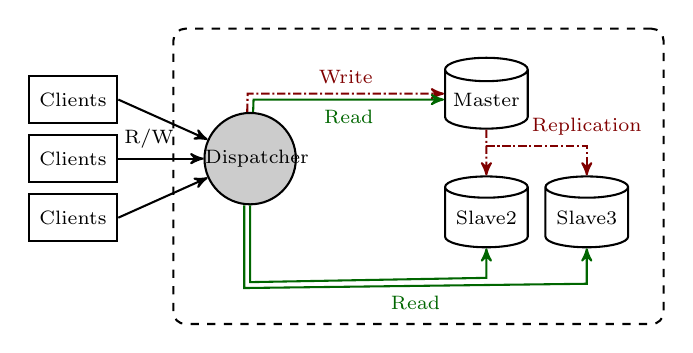
\begin{tikzpicture}
[font=\fontsize{6.75pt}{7.5}\selectfont, line width=0.75pt, node distance=0mm, draw=black, >=stealth',
server/.style={cylinder, shape border rotate=90, aspect=0.35, minimum height=9mm, minimum width=10.5mm, draw=black, inner sep=0pt},
client/.style={rectangle, minimum height=6mm, minimum width=11.25mm, draw=black, inner sep=0pt},
router/.style={circle, minimum size=11mm, draw=black, fill=gray!40, text width=3.25em, text centered, inner sep=0pt},
system/.style={rectangle, rounded corners=1.5mm, minimum height=37.5mm, minimum width=62.25mm, draw=black, dashed}
]

%MySQL system
\node[server](M) at (0,15mm) {Master};
\node[server](S2) at (0,0) {Slave2};
\node[server](S3) at (12.75mm,0) {Slave3};
\node[router](R) at (-30mm,7.5mm) {Dispatcher};
\node[system](MySQL) at (-8.625mm,5.25mm) {};

%Clients
\node[client](C1) at (-52.5mm,15mm) {Clients};
\node[client](C2) at (-52.5mm,7.5mm) {Clients};
\node[client](C3) at (-52.5mm,0) {Clients};

%write
\draw[->, color=black!50!red, densely dashdotted] ([xshift=-0.375mm]R.north) -- ([xshift=-24.9375mm,yshift=0.75mm]M.west) -- 
node[above, color=black!50!red] {Write} ([yshift=0.75mm]M.west);
%replication
\draw[->, color=black!50!red, densely dashdotted] (M.south) -- (S2.north);
\draw[->, color=black!50!red, densely dashdotted] ([yshift=3.75mm]S2.north) -- ([yshift=3.75mm]S3.north) node[above, color=black!50!red] {Replication} -- (S3.north);

%read
\draw[->, color=black!60!green] ([xshift=0.375mm]R.north) -- ([xshift=-24.1875mm]M.west) -- node[below, color=black!60!green] {Read} (M.west);
\draw[->, color=black!60!green] ([xshift=-0.75mm]R.south) -- ([xshift=-0.75mm,yshift=-10.5mm]R.south) -- 
node[below, color=black!60!green] {Read} ([yshift=-4.5mm]S3.south) -- (S3.south);
\draw[->, color=black!60!green] (R.south) -- ([yshift=-9.75mm]R.south) -- ([yshift=-3.75mm]S2.south) -- (S2.south);

%client request
\draw[->]  (C1.east) -- (R);
\draw[->]  (C2.east) -- node[left = 1.5mm, above, black] {R/W} (R);
\draw[->]  (C3.east) -- (R);

\end{tikzpicture}

\end{document}